% BDC223 Lecture 8: Chromatic Adaptation. Supplementary slides with TikZ figures.
% Data: Ramus et al. (1976b) Mar. Biol. 37: 223-229, Table 1 (light);
%       Ramus et al. (1976a) Mar. Biol. 37: 231-238, Figs 1-4 captions and Table I (pigments, rates);
%       Saffo (1987) BioScience 37: 654-664 (summary of mechanisms).
\documentclass[aspectratio=169,11pt]{beamer}
\usepackage[sfdefault,lining]{FiraSans}
\usepackage{amsmath}
\usefonttheme{professionalfonts}
\usepackage{firamath-otf}
\setmathrm{Fira Sans}
\usepackage{tikz}
\usepackage{pgfplots}
\pgfplotsset{compat=1.18}
\usetikzlibrary{arrows.meta,positioning}

\definecolor{ink}{HTML}{1F2A37}
\definecolor{accent}{HTML}{0F766E}
\definecolor{sea}{HTML}{1D4E89}
\definecolor{grey}{HTML}{6B7280}
\definecolor{leaf}{HTML}{3F8F2F}
\definecolor{warm}{HTML}{B45309}
\definecolor{rhodo}{HTML}{B91C1C}
\definecolor{shallow}{HTML}{F2B84B}
\definecolor{deep}{HTML}{1D4E89}
\setbeamercolor{frametitle}{fg=white,bg=ink}
\setbeamercolor{normal text}{fg=ink,bg=white}
\setbeamercolor{itemize item}{fg=accent}
\setbeamercolor{itemize subitem}{fg=accent}
\setbeamertemplate{itemize item}{\small$\blacktriangleright$}
\setbeamertemplate{itemize subitem}{\footnotesize\textendash}
\setbeamertemplate{navigation symbols}{}
\setbeamerfont{frametitle}{size=\Large,series=\bfseries}
\setbeamertemplate{frametitle}{%
  \nointerlineskip
  \begin{beamercolorbox}[wd=\paperwidth,ht=2.4em,dp=0.9em,leftskip=1.2em]{frametitle}
    \insertframetitle
  \end{beamercolorbox}}
\setbeamertemplate{footline}{%
  \hbox to \paperwidth{\hspace{1.2em}\color{grey}\tiny BDC223 Plant Ecophysiology \textbar{} Lecture 8: Chromatic Adaptation\hfill\insertframenumber\hspace{1.2em}}\vspace{0.6em}}
\setlength{\leftmargini}{1.4em}
\newcommand{\fignote}[1]{\par\vspace{2pt}{\color{grey}\scriptsize #1}}
\newcommand{\twocol}[2]{%
  \begin{columns}[c,onlytextwidth]
    \begin{column}{0.44\textwidth}#1\end{column}
    \begin{column}{0.54\textwidth}\centering #2\end{column}
  \end{columns}}

\tikzset{box/.style={draw=#1, very thick, rounded corners, fill=#1!7, text width=4.1cm, minimum height=3.3cm, align=flush left, inner sep=6pt}}
\hyphenpenalty=10000

\begin{document}

% 1 ---------------------------------------------------------------------
\begin{frame}{The light field at the study site}
\twocol{
\begin{itemize}
  \item Great Harbor, Woods Hole (USA), summer 1974--75
  \item Depth over which photon flux falls ten-fold:
  \begin{itemize}
    \item red 3.6 m; blue 5.3 m
    \item amber 6.0 m; green 6.0 m
  \end{itemize}
  \item At 10 m: 1.45\% of surface photons remain
  \item Coastal water turns the light \textbf{green-yellow}, not blue
  \item Depth reduces both \textbf{quantity} and \textbf{quality}
\end{itemize}}{
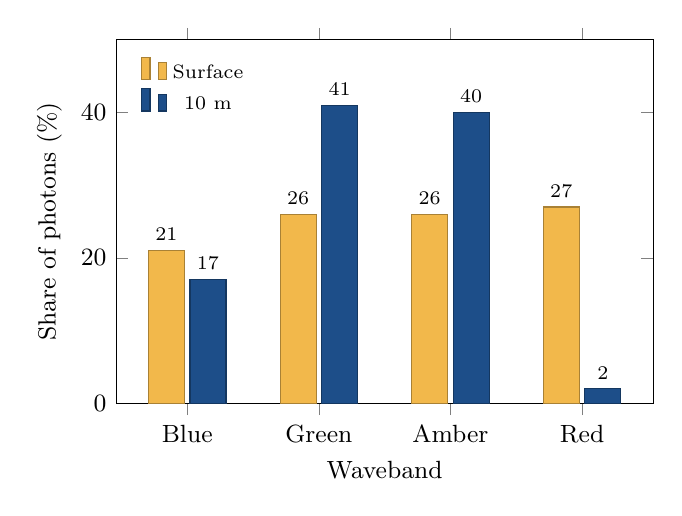
\begin{tikzpicture}
\begin{axis}[ybar, width=8.4cm, height=6.2cm, bar width=13pt, ymin=0, ymax=50,
  symbolic x coords={Blue,Green,Amber,Red}, xtick=data,
  xticklabel style={font=\small}, yticklabel style={font=\small},
  xlabel={\small Waveband}, ylabel={\small Share of photons (\%)},
  legend style={font=\scriptsize, at={(0.03,0.97)}, anchor=north west, draw=none, fill=none},
  nodes near coords, every node near coord/.append style={font=\scriptsize},
  enlarge x limits=0.18]
\addplot[fill=shallow, draw=shallow!70!black] coordinates {(Blue,21) (Green,26) (Amber,26) (Red,27)};
\addplot[fill=deep, draw=deep!70!black] coordinates {(Blue,17) (Green,41) (Amber,40) (Red,2)};
\legend{Surface, 10 m}
\end{axis}
\end{tikzpicture}
\fignote{Bands: blue 430--510, green 510--560, amber 560--620, red 620--710 nm. Data: Ramus et al. (1976b), Table 1.}}
\end{frame}

% 2 ---------------------------------------------------------------------
\begin{frame}{Pigment content after 7 days at 0.5 m or 10 m}
\twocol{
\begin{itemize}
  \item All four species made \textbf{more pigment} at 10 m
  \item \textit{Ulva}: about 9$\times$ more chl-\textit{a}; chl-\textit{b}:chl-\textit{a} 0.47 $\rightarrow$ 0.61
  \item \textit{Codium}: about 1.7$\times$ more chl-\textit{a}; chl-\textit{b}:chl-\textit{a} unchanged (0.65, 0.68)
  \item Red algae: phycoerythrin:chl-\textit{a} about doubled
  \item Changes reversed when lines were turned upside down
\end{itemize}}{
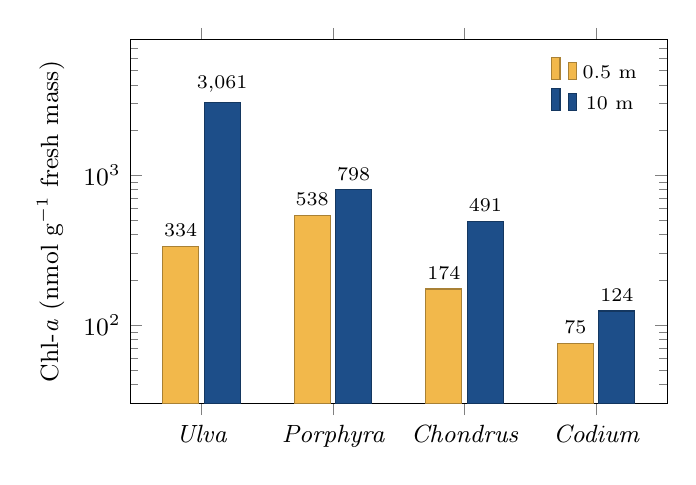
\begin{tikzpicture}
\begin{axis}[ybar, width=8.4cm, height=6.2cm, bar width=13pt, ymode=log, ymin=30, ymax=8000,
  log origin=infty,
  symbolic x coords={Ulva,Porphyra,Chondrus,Codium}, xtick=data,
  xticklabel style={font=\small\itshape}, yticklabel style={font=\small},
  ylabel={\small Chl-\textit{a} (nmol g$^{-1}$ fresh mass)},
  legend style={font=\scriptsize, at={(0.97,0.97)}, anchor=north east, draw=none, fill=none},
  nodes near coords, every node near coord/.append style={font=\scriptsize},
  point meta=rawy, enlarge x limits=0.18]
\addplot[fill=shallow, draw=shallow!70!black] coordinates {(Ulva,334) (Porphyra,538) (Chondrus,174) (Codium,75)};
\addplot[fill=deep, draw=deep!70!black] coordinates {(Ulva,3061) (Porphyra,798) (Chondrus,491) (Codium,124)};
\legend{0.5 m, 10 m}
\end{axis}
\end{tikzpicture}
\fignote{Log scale. Data: Ramus et al. (1976a), Figs 1--4 captions; reversal: Ramus et al. (1976b).}}
\end{frame}

% 3 ---------------------------------------------------------------------
\begin{frame}{Light-saturated photosynthesis per unit chlorophyll-\textit{a}}
\twocol{
\begin{itemize}
  \item Laboratory rates at saturating light
  \item \textit{Ulva}: rate per chl-\textit{a} fell to one third at 10 m
  \begin{itemize}
    \item extra chlorophyll enlarges the antennae, not the capacity to use bright light
  \end{itemize}
  \item Other species: changes within about 25\%
  \item Deep \textit{Ulva} and \textit{Codium} saturated at half the irradiance
\end{itemize}}{
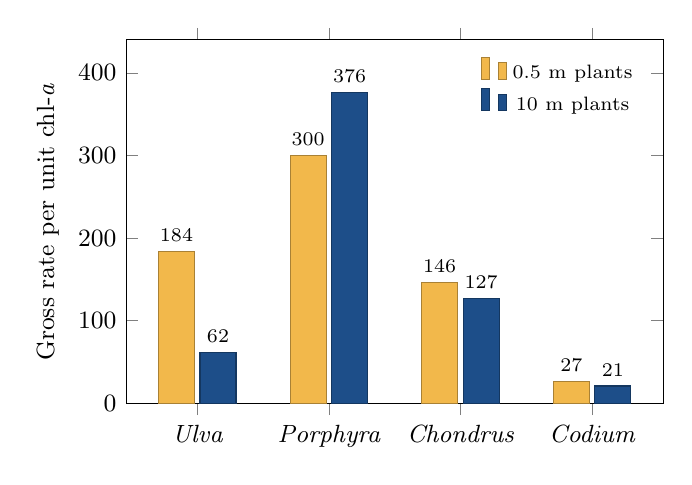
\begin{tikzpicture}
\begin{axis}[ybar, width=8.4cm, height=6.2cm, bar width=13pt, ymin=0, ymax=440,
  symbolic x coords={Ulva,Porphyra,Chondrus,Codium}, xtick=data,
  xticklabel style={font=\small\itshape}, yticklabel style={font=\small},
  ylabel={\small Gross rate per unit chl-\textit{a}},
  legend style={font=\scriptsize, at={(0.97,0.97)}, anchor=north east, draw=none, fill=none},
  nodes near coords, every node near coord/.append style={font=\scriptsize},
  enlarge x limits=0.18]
\addplot[fill=shallow, draw=shallow!70!black] coordinates {(Ulva,184) (Porphyra,300) (Chondrus,146) (Codium,27)};
\addplot[fill=deep, draw=deep!70!black] coordinates {(Ulva,62) (Porphyra,376) (Chondrus,127) (Codium,21)};
\legend{0.5 m plants, 10 m plants}
\end{axis}
\end{tikzpicture}
\fignote{Units as in Ramus et al. (1976a), Table I; 26\,\textdegree C, 10 mW cm$^{-2}$.}}
\end{frame}

% 4 ---------------------------------------------------------------------
\begin{frame}{Three ways to harvest dim, green light}
\begin{center}
\vspace*{-6pt}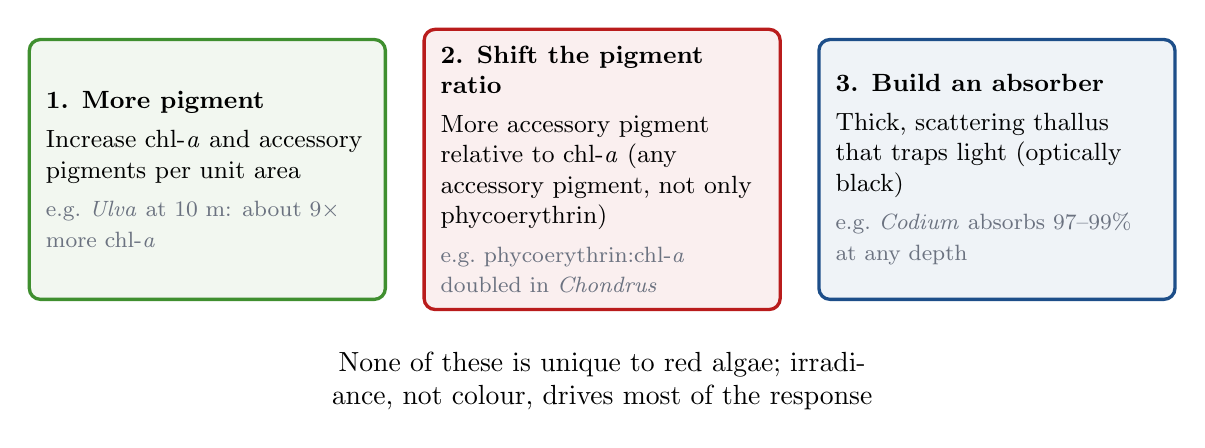
\begin{tikzpicture}[font=\small]
  \node[box=leaf] (a) at (0,0) {\textbf{1. More pigment}\\[3pt] Increase chl-\textit{a} and accessory pigments per unit area\\[3pt]{\color{grey}\footnotesize e.g.\ \textit{Ulva} at 10 m: about 9$\times$ more chl-\textit{a}}};
  \node[box=rhodo, right=0.45cm of a] (b) {\textbf{2. Shift the pigment ratio}\\[3pt] More accessory pigment relative to chl-\textit{a} (any accessory pigment, not only phycoerythrin)\\[3pt]{\color{grey}\footnotesize e.g.\ phycoerythrin:chl-\textit{a} doubled in \textit{Chondrus}}};
  \node[box=sea, right=0.45cm of b] (c) {\textbf{3. Build an absorber}\\[3pt] Thick, scattering thallus that traps light (optically black)\\[3pt]{\color{grey}\footnotesize e.g.\ \textit{Codium} absorbs 97--99\% at any depth}};
  \node[below=0.4cm of b, text width=13cm, align=center, font=\normalsize] {None of these is unique to red algae; irradiance, not colour, drives most of the response};
\end{tikzpicture}
\end{center}
\vspace{-4pt}\fignote{After Saffo (1987); data from Ramus et al. (1976a) and Ramus (1978).}
\end{frame}

\end{document}
